Реализация метода \textit{Time of Flight} заключается в следующем: радиоволна летит от источника к приёмнику, который работает в режиме ретранслятора. Приёмник отправляет сигнал назад источнику, который фиксирует время полёта сигнала. Поделив это время на 2, получим время полёта сигнала от источника к приёмнику (формула~\eqref{eq:timeflight}):

\begin{equation}
    \label{eq:timeflight}
    t = \frac{T_f}{2},
\end{equation}

где $T_f$ --- время полёта (flight) от источника к приёмнику и обратно.

На рисунке~\ref{fig:tofscheme} представлена функциональная схема такого устройства.

\begin{figure}[ht]
    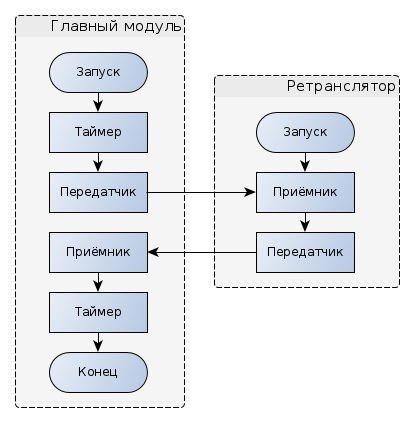
\includegraphics[width=.65\linewidth]{Figures/tofscheme.png}
    \caption{Функциональная схема устройства \textit{Time of Flight}}
    \label{fig:tofscheme}
\end{figure}

Электромагнитное излучение преодолевает расстояние со скоростью около 300.000.000 м/с. Таким образом, чтобы успеть <<словить>> время пролёта электромагнитной волны, детектор должен работать на частоте, равной или превышающей время пролёта сигнала от источника к приёмнику и обратно (формула~\eqref{eq:freqflight}). Чем более высокой будет частота работы устройства, тем больше будет его разрешающая способность и тем более точные результаты мы получим.

\begin{equation}
    \label{eq:freqflight}
    f = \frac{1}{T_f} = \frac{c}{S},
\end{equation}

где c --- скорость света, S --- минимально возможное расстояние, на котором прибор с данной частотой должен успевать уловить время $T_f$ полёта радиоволны.

Таким образом, для обеспечения работы на расстоянии в 3 метра, устройство должно работать на частоте как минимум $f = \frac{300.000.000}{3} = 100$ МГц. Для 300 метров --- 1 МГц.

Для уменьшения необходимой частоты работы устройства, а также сокращению возможных погрешностей и ошибок, воспользуемся методом <<накопления>> ToF.
